\subsubsection{Throughput comparison}
\begin{frame}{\subsecname: \subsubsecname}
    \begin{figure}
        \centering
        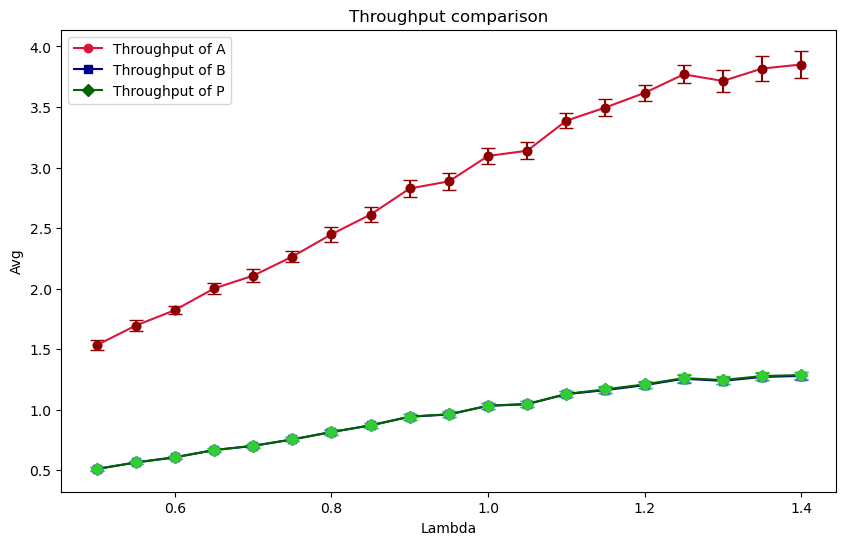
\includegraphics[width=0.75\linewidth]{figs/results/obj4/obj4-throughput-comparison.png}
        \caption{Confronto tra throughput dei tre server con tasso di arrivo $1.4 job/s$}
        \label{fig:enter-label}
    \end{figure}
\end{frame}

\subsubsection{Service time from 0.8 to 0.4}
\begin{frame}{\subsecname: \subsubsecname}
    \begin{figure}
        \centering
        \begin{subfigure}{0.49\linewidth}
            \centering
            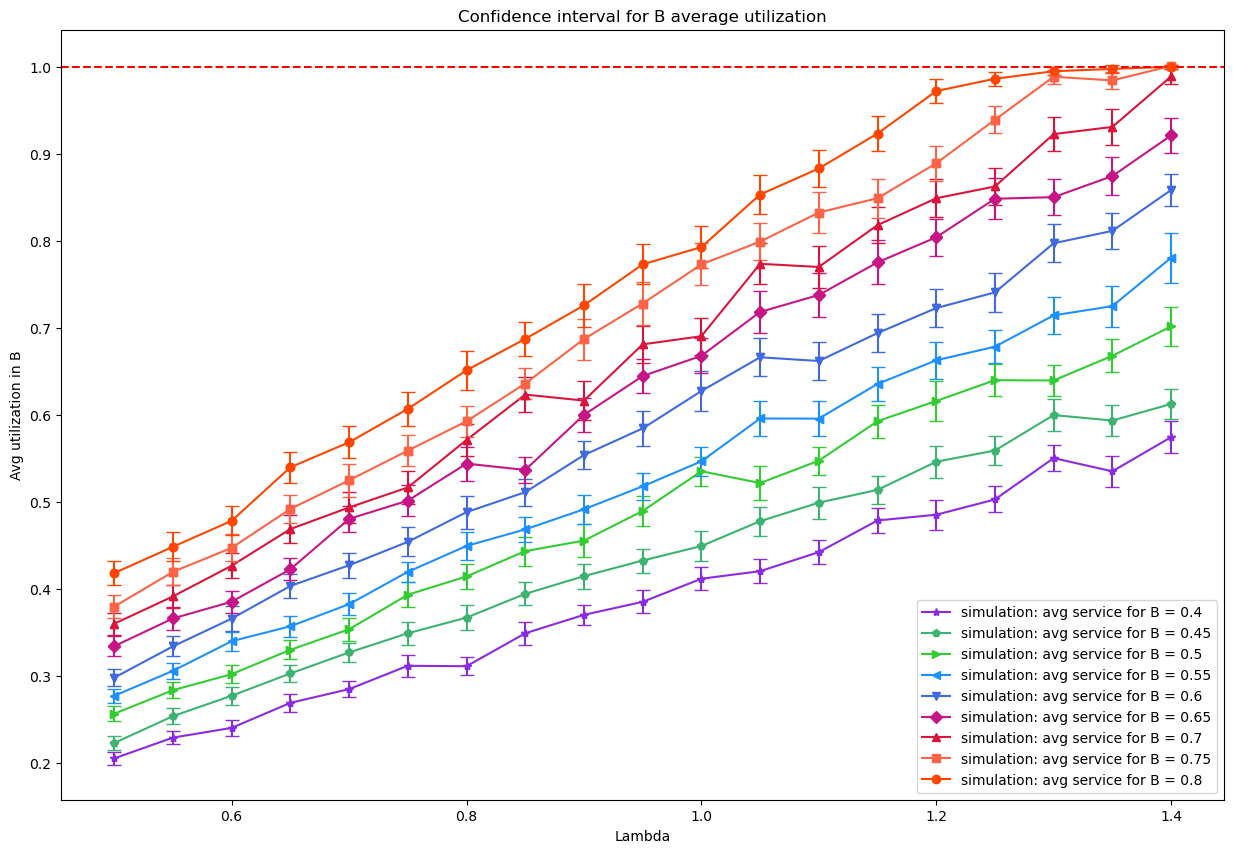
\includegraphics[width=\linewidth]{figs/results/obj4/obj4-utilization-service-time.png}
            \caption{Utilizzazione}
            \label{fig:obj4_utilization_service-time}
        \end{subfigure}
        \hfill
        \begin{subfigure}{0.49\linewidth}
            \centering
            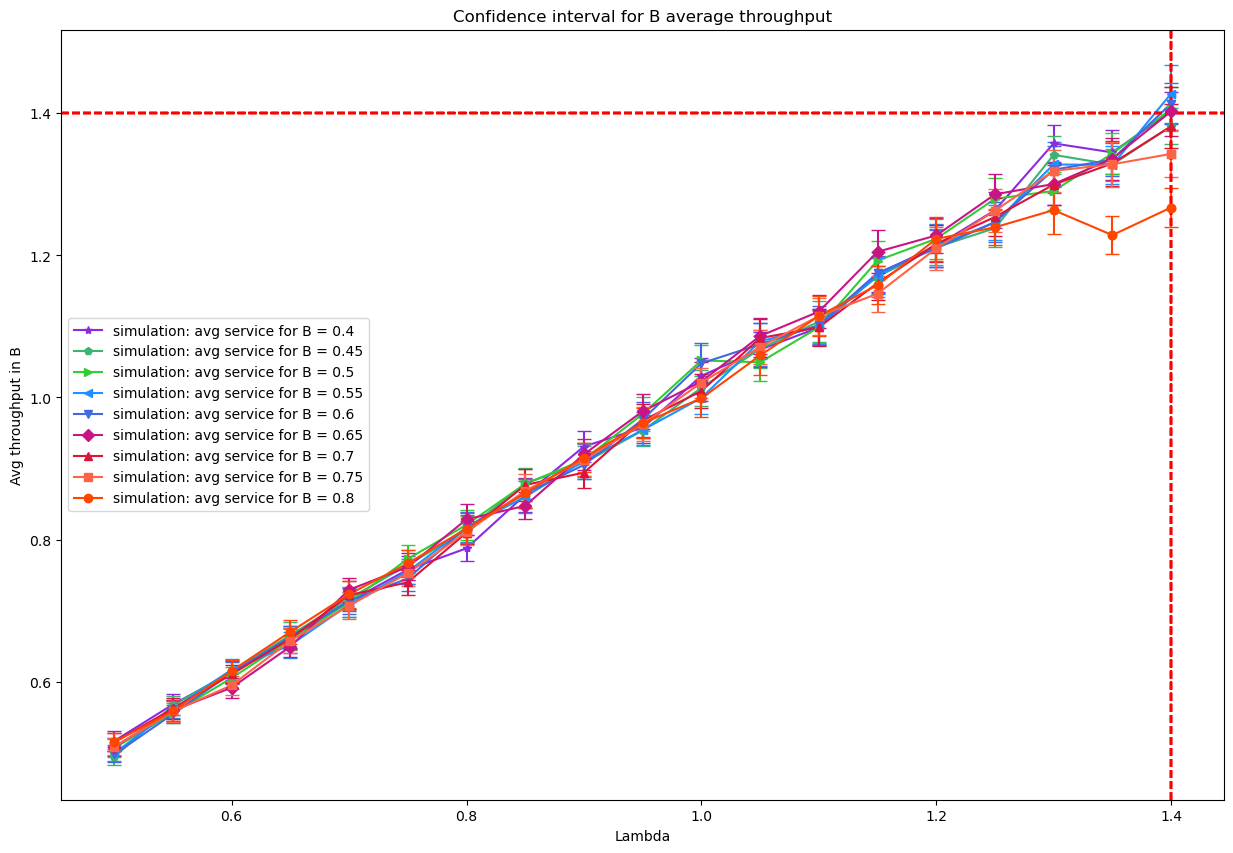
\includegraphics[width=\linewidth]{figs/results/obj4/obj4-throughput-service-time.png}
            \caption{Throughput}
            \label{fig:obj4_throughput_service-time}
        \end{subfigure}
        \caption{Confronto Throughput e Utilizzazione medi al variare dei valori dei tempi di servizio}
        \label{fig:obj4-service-time-comparison}
    \end{figure}
\end{frame}

\subsubsection{Service time 0.4 vs 0.65}
\begin{frame}{\subsecname: \subsubsecname}
    \begin{table}
        \centering
        \begin{tabularx}{\textwidth}{X X}
            \begin{minipage}{0.48\textwidth}
                \centering
                \caption{Minimi e massimi di utilizzazione e throughput per tempi di servizio 0.65 del server B}
                \begin{tabular}{ccc}
                    $\lambda$ & metrica & valore\\
                    0.5 & utilizzazione & 0.333898\\
                    1.4 & utilizzazione & 0.921304\\
                    0.5 & throughput & 0.507752\\
                    1.4 & throughput & 1.40273
                \end{tabular}
                \label{tab:065_metrics}
            \end{minipage}
            &
            \begin{minipage}{0.48\textwidth}
                \centering
                \caption{Minimi e massimi di utilizzazione e throughput per tempi di servizio 0.4 del server B}
                \begin{tabular}{ccc}
                    $\lambda$ & metrica & valore\\
                    0.5 & utilizzazione & 0.20484\\
                    1.4 & utilizzazione & 0.574275\\
                    0.5 & throughput & 0.516347\\
                    1.4 & throughput & 1.40302
                \end{tabular}
                \label{tab:04_metrics}
            \end{minipage}
        \end{tabularx}
    \end{table}
\end{frame}

\subsubsection{Finite Horizion (service time 0.4)}
\begin{frame}{\subsecname: \subsubsecname}
    \begin{figure}
        \centering
        \begin{subfigure}{\linewidth}
            \centering
            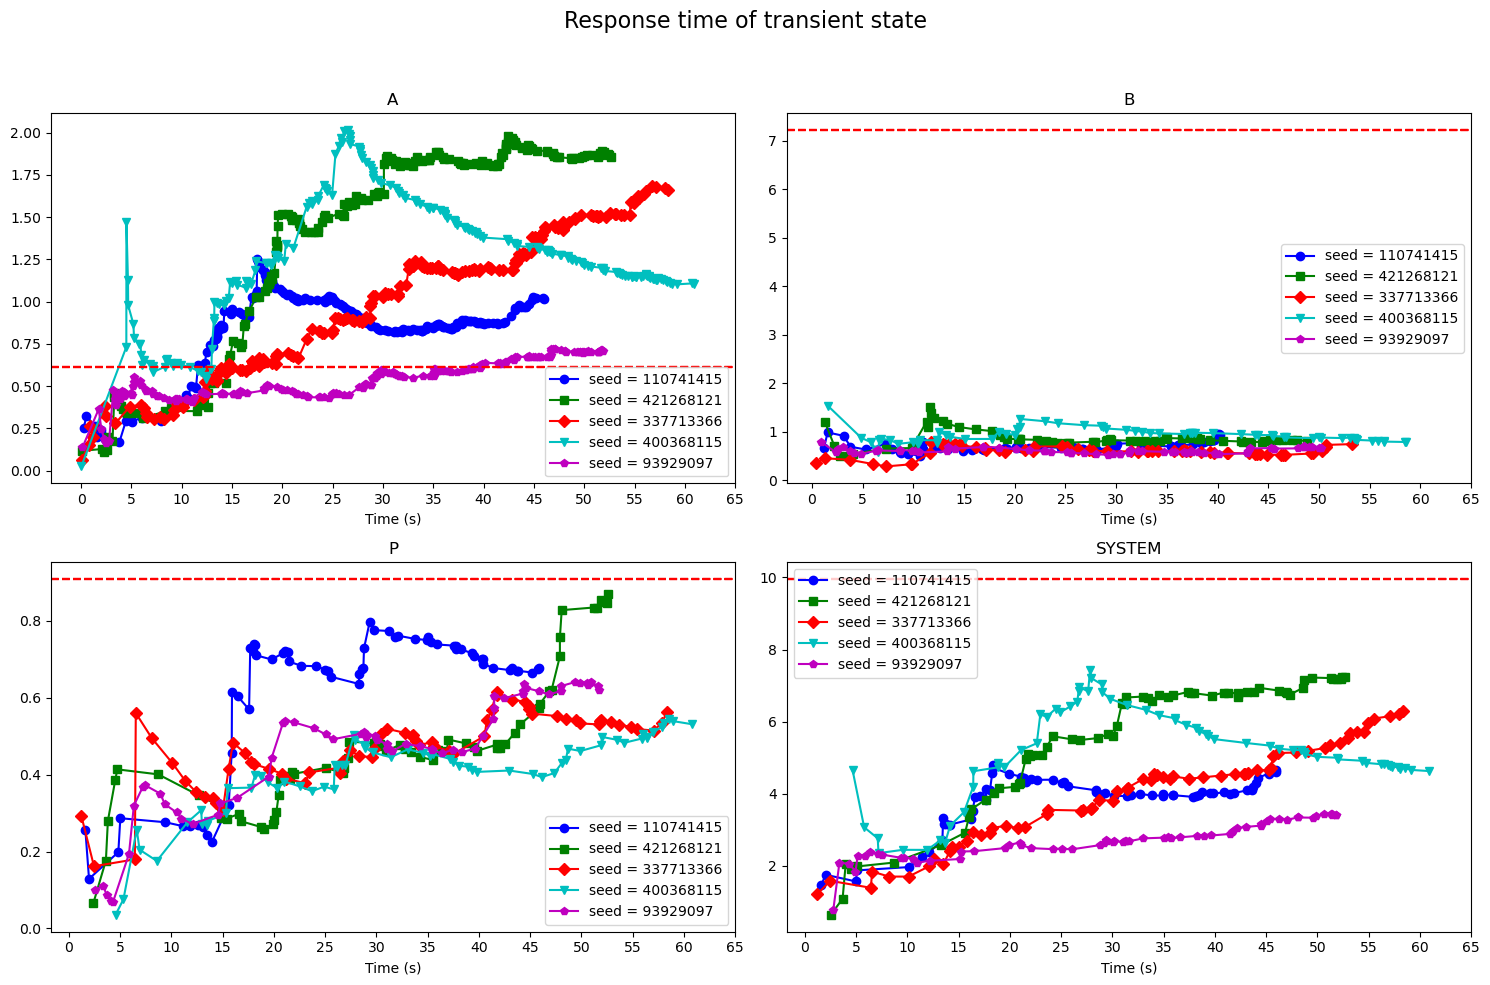
\includegraphics[width=0.8\linewidth]{figs/appendices/transient/obj4_04-transient-rtime-analitycal.png}
            \caption{Senza valore analitico}
            \label{fig:obj4_04_transient_simulation}
            \end{subfigure} 
        \begin{subfigure}{\linewidth}
            \centering
            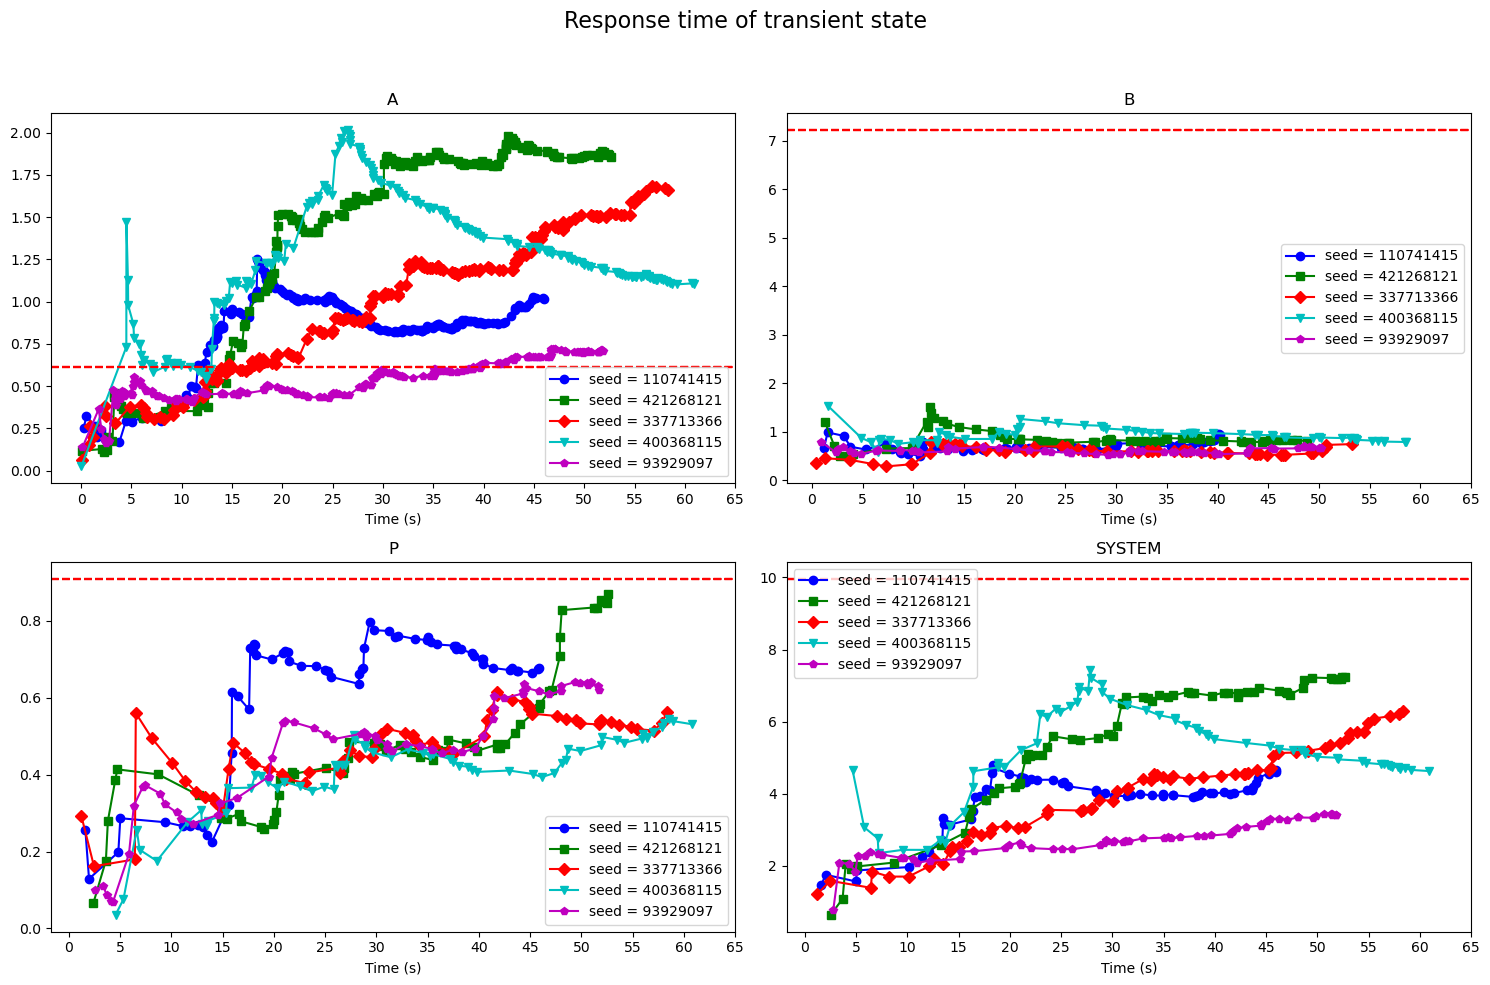
\includegraphics[width=0.8\linewidth]{figs/appendices/transient/obj4_04-transient-rtime-analitycal.png}
            \caption{Con valore analitico}
            \label{fig:obj4_04_transient_analitycal}
            \end{subfigure}
        \caption{Tempo di risposta per l'obiettivo 4 (con il server B con tempi di servizio 0.4s) in funzione del tempo di simulazione nello stato transiente del sistema con un rate di arrivi 1.4$job/s$ al variare del seed.}
        \label{fig:obj4_04_transient}
    \end{figure}
\end{frame}


\subsubsection{Verification (service time 0.4)}
\begin{frame}{\subsecname: \subsubsecname}
    \begin{figure}
        \centering
        \begin{subfigure}{0.35\linewidth}
            \centering
            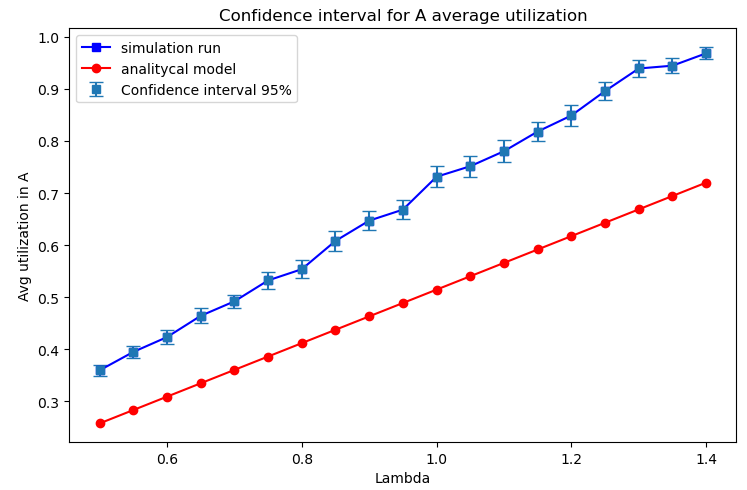
\includegraphics[width=\linewidth]{figs/results/obj4/obj4-utilizzazione-A.png}
            \label{fig:obj4_line_utilization_A}
        \end{subfigure} 
        \begin{subfigure}{0.35\linewidth}
            \centering
             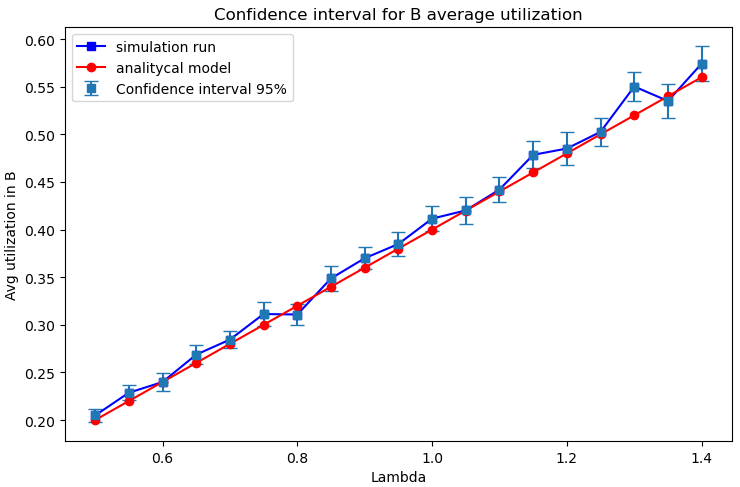
\includegraphics[width=\linewidth]{figs/results/obj4/obj4-utilizzazione-B.png}
            \label{fig:obj4_line_utilization_B}
        \end{subfigure}
        \begin{subfigure}{0.35\linewidth}
            \centering
            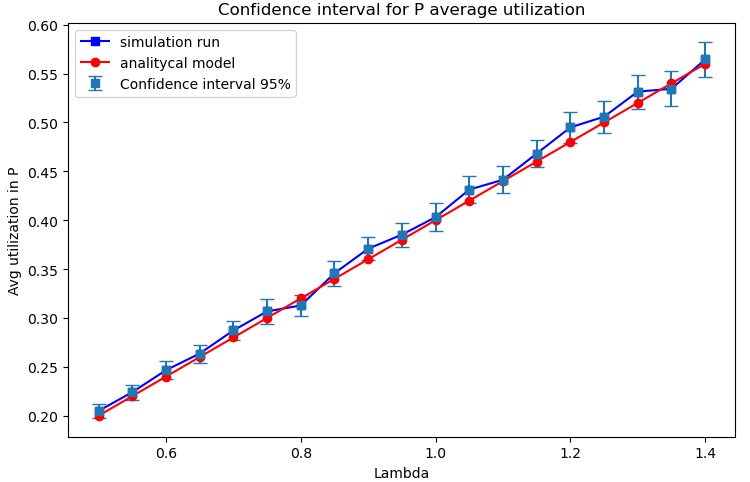
\includegraphics[width=\linewidth]{figs/results/obj4/obj4-utilizzazione-P.png}
            \label{fig:obj4_line_utilization_P}
        \end{subfigure}
        \caption{Intervallo di confidenza dell'utilizzazione e confronto con modello analitico per l'obiettivo 4.}
        \label{fig:obj4_lineplots_utilization}
    \end{figure}   
\end{frame}

\subsubsection{Validation}
\begin{frame}{\subsecname: \subsubsecname}
    \begin{figure}
        \centering
        \begin{subfigure}[b]{0.49\textwidth}
            \centering
            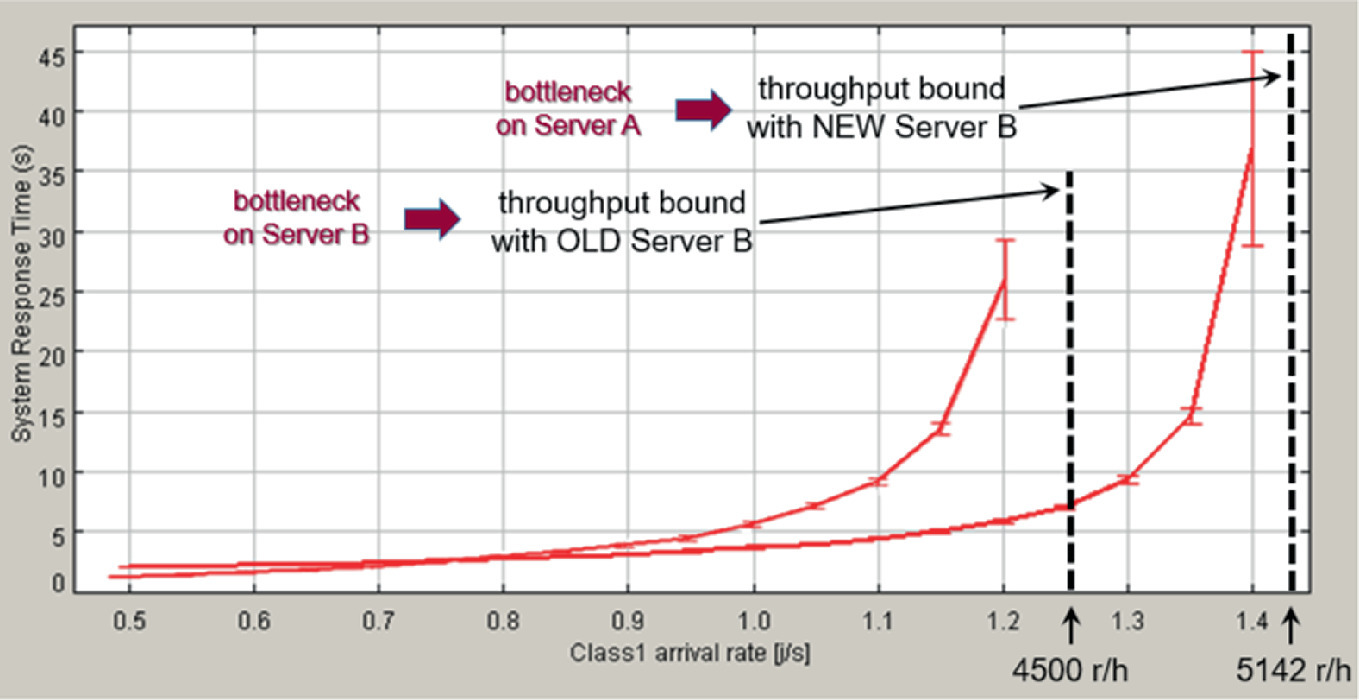
\includegraphics[width=\columnwidth]{figs/results/obj4/obj4-validazione.jpg}
            \caption{Caso di studio \citep{DBLP:books/sp/Serazzi24}}
            \label{fig:obj4_validazione_casestudy}
        \end{subfigure}
        \begin{subfigure}[b]{0.49\textwidth}
            \centering
            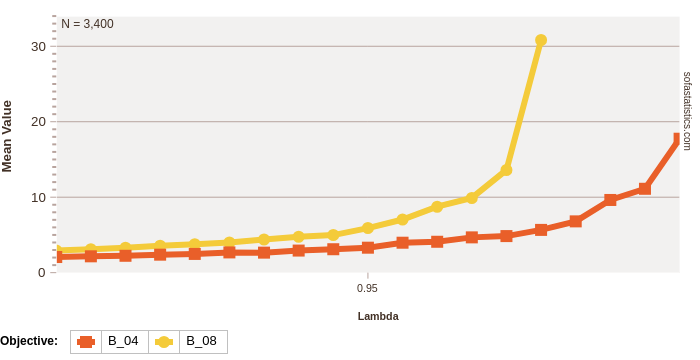
\includegraphics[width=\columnwidth]{figs/results/obj4/obj4-simulazione-validazione.png}
            \caption{Risultati sperimentali}
            \label{fig:obj4_validazione_simulation}
        \end{subfigure}
        \hfill
        \caption{Tempo di risposta medio prima e dopo la miglioria del server B in funzione del rate medio degli arrivi esterni}
        \label{fig:obj4_validazione}
    \end{figure}
\end{frame}
